\chapter{Robust MPC and Tube MPC\texorpdfstring{$^{(*)}$}{(*)}}
\label{chap:tube_mpc}

\begin{quote}
	\textit{``Standard MPC tells you the best thing to do if the world is perfect. Tube MPC tells you what to do when it isn't.''} \\
	\hfill --- paraphrasing \textbf{David Q.\ Mayne}
\end{quote}

Every MPC formulation we have seen so far relies on a perfect model: $x_{k+1} = Ax_k + Bu_k$. The controller solves an optimisation, applies the first input, and re-solves at the next step. This works well in practice --- \emph{provided the model is accurate}. In practice, however, systems are always subject to disturbances: sensor noise, wind gusts, friction that the model ignores, or small inaccuracies in the $A$ and $B$ matrices themselves. Even a tiny modelling error, accumulated over many steps, can push the real state across a constraint boundary that the controller thought was safe.

This chapter addresses the question: \textbf{how do we guarantee constraint satisfaction when the model is not perfect?} The answer is \emph{robust MPC}, and the most practical and widely-used form is called \textbf{Tube MPC}, introduced by Langson et al.~\cite{Langson2004} and further developed by Mayne et al.~\cite{Mayne2005}. The central idea is straightforward: instead of planning a single trajectory, we plan a ``tube'' of trajectories. As long as the disturbance is bounded, the real trajectory stays inside the tube, and the tube is designed so that constraints are never violated.

\section{The Problem: Disturbances and Constraint Violations}
\label{sec:tube_problem}

Consider the linear system with an additive disturbance:
\begin{equation} \label{eq:uncertain_system}
	x_{k+1} = Ax_k + Bu_k + w_k
\end{equation}
where $x_k \in \mathbb{R}^n$ is the state, $u_k \in \mathbb{R}^m$ is the control input, and $w_k \in \mathbb{R}^n$ is a disturbance. We assume:
\begin{itemize}[noitemsep]
	\item The disturbance is bounded: $w_k \in \mathcal{W}$ for all $k \ge 0$, where $\mathcal{W}$ is a known convex polytope containing the origin (e.g., $\|w_k\|_\infty \le \delta$ for some known $\delta > 0$).
	\item We do \emph{not} know the specific value of $w_k$ in advance. We only know it will lie somewhere in $\mathcal{W}$.
\end{itemize}

The system is subject to constraints:
\[
x_k \in \mathcal{X}, \qquad u_k \in \mathcal{U}, \qquad \text{for all } k \ge 0
\]

\subsection*{Why Standard MPC Fails}

Standard MPC ignores $w_k$ and plans as if $x_{k+1} = Ax_k + Bu_k$. At each step, it re-measures the state and re-solves, which provides some natural robustness. However, this is not enough to \emph{guarantee} constraint satisfaction.

Suppose the MPC plans a trajectory that passes close to a constraint boundary --- say $x_1 \le 5$. The controller predicts $x_1 = 4.95$ and decides this is safe. But after the input is applied, the disturbance $w_0$ adds an unexpected $+0.1$ to the state, producing $x_1 = 5.05$. The constraint is violated.

Standard MPC cannot prevent this because it does not account for the ``worst case'' during planning. It optimistically assumes the prediction is exact.

\begin{alertbox}{The core difficulty}
	Standard MPC guarantees constraints are satisfied for the \emph{predicted} trajectory. But when disturbances act, the \emph{actual} trajectory deviates from the prediction. No amount of re-solving at the next step can undo a constraint violation that has already occurred.
\end{alertbox}

\section{Two Approaches to Robust MPC}

Two main approaches exist for handling bounded disturbances.

\subsection{Min--Max MPC}

The most direct approach formulates the problem as a game between the controller and an adversary (nature). The controller chooses inputs $u$ to minimise the cost, while nature chooses disturbances $w \in \mathcal{W}$ to maximise it:
\[
\min_{u_0, \ldots, u_{N-1}} \;\max_{w_0, \ldots, w_{N-1} \in \mathcal{W}} \; J(x, u)
\]
subject to the dynamics~\eqref{eq:uncertain_system} and the constraints $x_k \in \mathcal{X}$, $u_k \in \mathcal{U}$ for all possible disturbance realisations.

This is mathematically rigorous but has serious drawbacks:
\begin{itemize}[noitemsep]
	\item \textbf{Computational explosion.} The disturbance branches at every time step. Over $N$ steps with $d$ possible disturbance vertices, the number of scenarios grows as $d^N$. For even modest problems, this becomes intractable.
	\item \textbf{Conservatism.} The controller assumes nature is adversarial and always picks the worst disturbance. In reality, disturbances are often random, not adversarial. The resulting controller is overly cautious.
\end{itemize}

Min--max MPC is therefore rarely used in practice. It is included here for completeness and to motivate the more practical alternative.

\subsection{Tube MPC: The Key Idea}

Tube MPC avoids the computational explosion by separating the problem into two parts:
\begin{enumerate}
	\item A \textbf{nominal trajectory} $z_k$ that is planned as if there were no disturbance. This is a standard MPC problem.
	\item A \textbf{feedback controller} $-K(x_k - z_k)$ that keeps the real state $x_k$ close to the nominal trajectory $z_k$, despite the disturbance.
\end{enumerate}

\begin{notebox}{Notation: $z_k$ in This Chapter}
	Throughout this chapter, $z_k$ denotes the \textbf{nominal state} (the disturbance-free planned trajectory). This is unrelated to the augmented state vector $z_k = [x_k^\top\;\; d_k^\top]^\top$ used in the offset-free MPC formulation of Chapter~\ref{chap:output_fb_mpc}. The two uses of $z_k$ never appear in the same context.
\end{notebox}

The deviation $e_k = x_k - z_k$ between the real and nominal state is bounded because $K$ is stabilising and the disturbance is bounded. The set of all possible deviations forms a ``tube'' around the nominal trajectory. By tightening the constraints on the nominal trajectory (shrinking them inward by the tube width), we guarantee that the real trajectory satisfies the original constraints.

This is the essence of Tube MPC: \textbf{plan the nominal path conservatively, and let a feedback controller handle the disturbances.}

\section{Set Operations: Minkowski Sum and Pontryagin Difference}

Before developing Tube MPC formally, we need two set operations that appear throughout the theory. These are not difficult, but they are essential.

\subsection{Minkowski Sum}

\begin{defnbox}{Definition: Minkowski Sum}
	The \textbf{Minkowski sum} of two sets $P$ and $Q$ in $\mathbb{R}^n$ is:
	\[
	P \oplus Q = \{p + q \mid p \in P, \; q \in Q\}
	\]
	In words: take every point in $P$, add every point in $Q$, and collect all the results. The resulting set is ``$P$ inflated by $Q$''.
\end{defnbox}

\textbf{Geometric intuition.} Place a copy of $Q$ at every point of $P$. The Minkowski sum is the union of all these copies. If $P$ is a square and $Q$ is a small disk, then $P \oplus Q$ is the square with rounded corners. Figure~\ref{fig:minkowski_sum} illustrates this operation.

\begin{figure}[H]
	\centering
	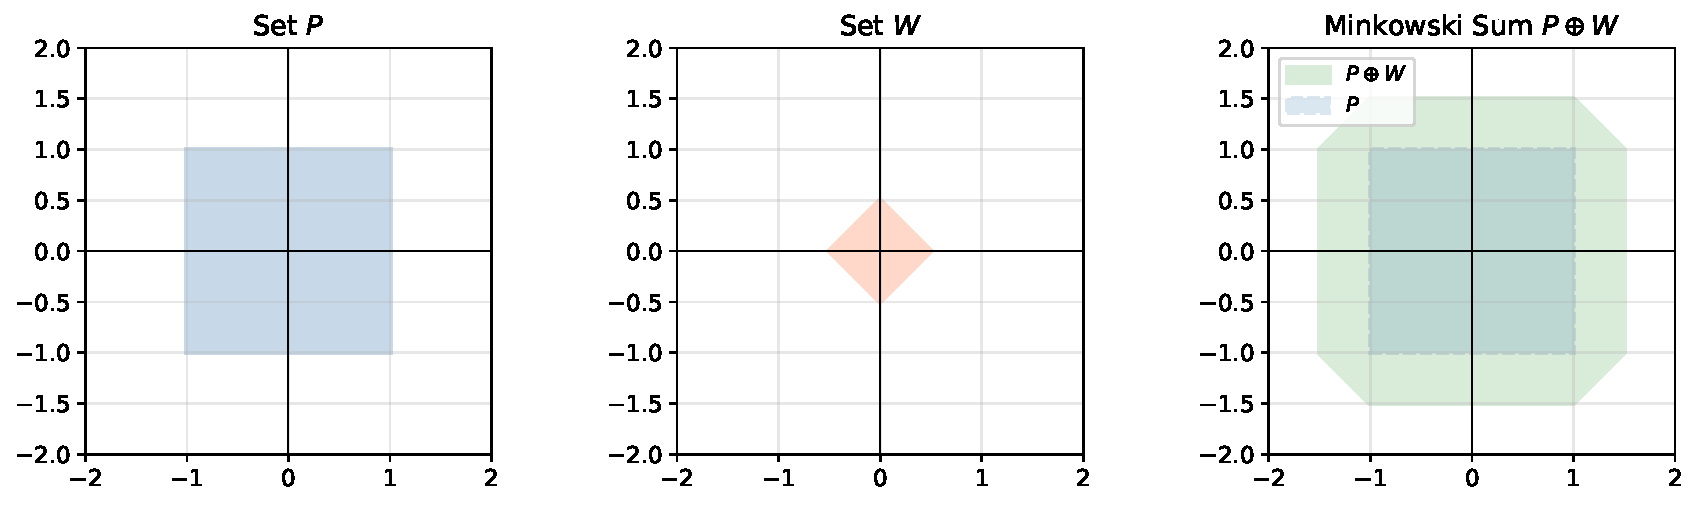
\includegraphics[width=0.95\linewidth]{Figures/minkowski_sum.pdf}
	\caption{Minkowski sum of a square $P$ and a diamond $W$. The result $P \oplus W$ is larger than $P$, ``inflated'' by the shape of $W$.}
	\label{fig:minkowski_sum}
\end{figure}

\textbf{Why it matters for Tube MPC.} If the nominal state is $z_k$ and the error $e_k$ can be anywhere in a set $\mathcal{E}$, then the actual state $x_k = z_k + e_k$ can be anywhere in $\{z_k\} \oplus \mathcal{E}$. The tube around the nominal trajectory is exactly this: the Minkowski sum of each nominal point with the error set.

\subsection{Pontryagin Difference}

\begin{defnbox}{Definition: Pontryagin Difference}
	The \textbf{Pontryagin difference} (also called the \emph{erosion}) of a set $\mathcal{X}$ by a set $\mathcal{E}$ is:
	\[
	\mathcal{X} \ominus \mathcal{E} = \{z \in \mathbb{R}^n \mid z + e \in \mathcal{X} \;\; \text{for all } e \in \mathcal{E}\}
	\]
	In words: $\mathcal{X} \ominus \mathcal{E}$ contains all points $z$ such that \emph{every possible shift by an element of $\mathcal{E}$} still lands inside $\mathcal{X}$.
\end{defnbox}

\textbf{Geometric intuition.} The Pontryagin difference is the ``shrunk'' version of $\mathcal{X}$. If you stand at a point $z \in \mathcal{X} \ominus \mathcal{E}$ and someone pushes you by any amount in $\mathcal{E}$, you still remain inside $\mathcal{X}$. It is the opposite of the Minkowski sum: while $\oplus$ inflates a set, $\ominus$ shrinks it. See Figure~\ref{fig:pontryagin_diff} for an illustration.

\begin{figure}[H]
	\centering
	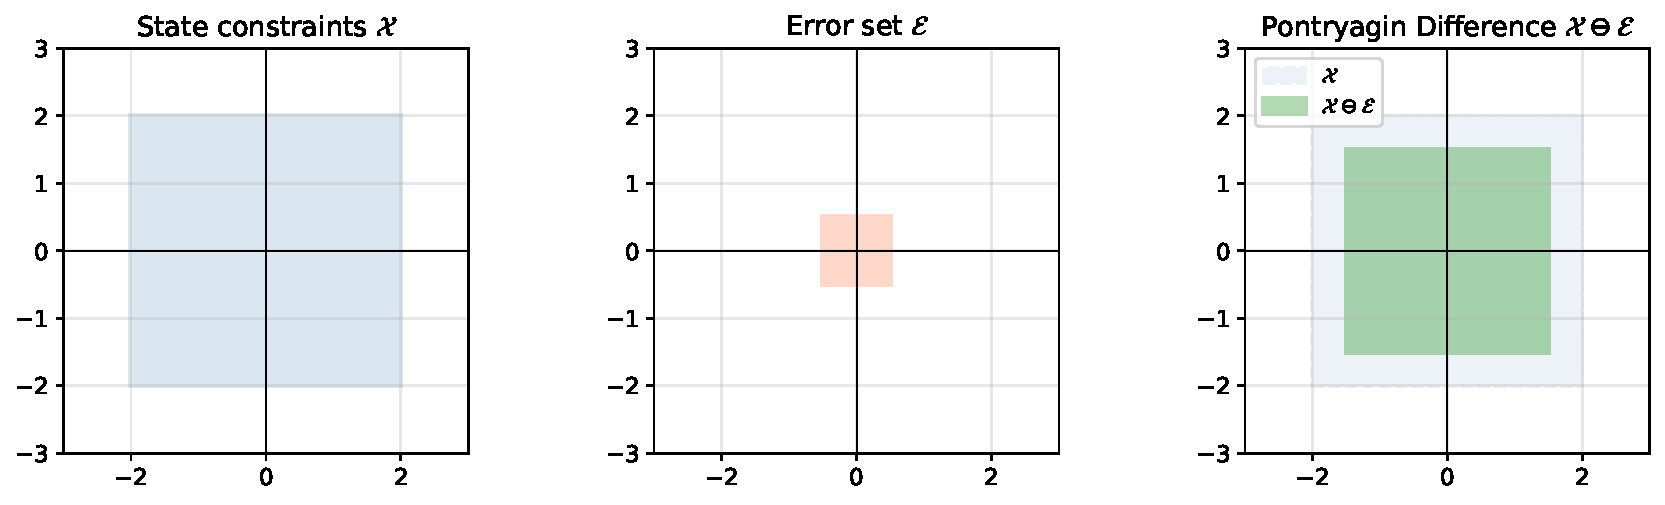
\includegraphics[width=0.95\linewidth]{Figures/pontryagin_diff.pdf}
	\caption{Pontryagin difference $\mathcal{X} \ominus \mathcal{E}$. The original constraint set $\mathcal{X}$ (dashed blue) is shrunk inward by the size of $\mathcal{E}$ (red), yielding the tightened set (solid green). Any point in the tightened set remains inside $\mathcal{X}$ even after a worst-case shift from $\mathcal{E}$.}
	\label{fig:pontryagin_diff}
\end{figure}

\textbf{Why it matters for Tube MPC.} To guarantee that the real state $x_k = z_k + e_k$ satisfies $x_k \in \mathcal{X}$ for all $e_k \in \mathcal{E}$, we must require the nominal state to satisfy $z_k \in \mathcal{X} \ominus \mathcal{E}$. This is called \emph{constraint tightening}.

\begin{examplebox}{Minkowski Sum and Pontryagin Difference in 1D}
	Let $\mathcal{X} = [-5, \; 5]$ (the state must stay between $-5$ and $5$) and $\mathcal{E} = [-0.3, \; 0.3]$ (the error is at most $0.3$ in magnitude).

	\solution

	\textbf{Minkowski sum:} $\mathcal{X} \oplus \mathcal{E} = [-5.3, \; 5.3]$. The set grows by the error width on each side.

	\textbf{Pontryagin difference:} $\mathcal{X} \ominus \mathcal{E} = [-4.7, \; 4.7]$. The set shrinks by $0.3$ on each side. If the nominal state $z$ stays within $[-4.7, 4.7]$, then $x = z + e$ stays within $[-5, 5]$ for any $|e| \le 0.3$.

	This is constraint tightening: the nominal trajectory must respect the stricter bounds $\pm 4.7$, so that the actual trajectory respects the original bounds $\pm 5$.
\end{examplebox}


\section{Tube MPC: The Full Development}
\label{sec:tube_full}

We now develop Tube MPC step by step.

\subsection{Step 1: Decompose the System}

The uncertain system is $x_{k+1} = Ax_k + Bu_k + w_k$. We introduce a \emph{nominal} system that evolves without disturbance:
\begin{equation} \label{eq:nominal_system}
	z_{k+1} = Az_k + Bv_k
\end{equation}
where $z_k$ is the nominal state and $v_k$ is the nominal input. These are the decision variables that the MPC optimiser will compute.

We define the \emph{error} between the real and nominal states:
\[
e_k = x_k - z_k
\]

The control input is split into two parts:
\begin{equation} \label{eq:tube_control_law}
	u_k = v_k - K(x_k - z_k) = v_k - Ke_k
\end{equation}
where:
\begin{itemize}[noitemsep]
	\item $v_k$ is the \textbf{nominal input}, computed by the MPC optimiser. It steers the nominal trajectory $z_k$ toward the origin.
	\item $K$ is a \textbf{fixed feedback gain} (typically the LQR gain from \texttt{dlqr}, so $K > 0$ and $u = -Kx$ stabilises the system). It keeps the real state close to the nominal state by rejecting disturbances.
\end{itemize}

\subsection{Step 2: Derive the Error Dynamics}

Substituting~\eqref{eq:tube_control_law} into the real dynamics~\eqref{eq:uncertain_system} and subtracting the nominal dynamics~\eqref{eq:nominal_system}:

\begin{align*}
	x_{k+1} &= Ax_k + B(v_k - Ke_k) + w_k \\
	z_{k+1} &= Az_k + Bv_k
\end{align*}

Subtracting:
\begin{equation} \label{eq:error_dynamics}
	\boxed{e_{k+1} = (A - BK)\,e_k + w_k}
\end{equation}

This is the key result. The error dynamics are \emph{autonomous}: they do not depend on $v_k$ at all. The nominal input cancels out. The error evolves purely under the closed-loop matrix $A_{cl} = A - BK$ and the disturbance $w_k$.

Since $K$ is chosen so that $A_{cl}$ is Schur stable (all eigenvalues inside the unit circle), the error $e_k$ does not grow without bound. But it does not converge to zero either, because the disturbance $w_k$ keeps pushing it around. Instead, $e_k$ settles into a bounded set that we can compute.

\subsection{Step 3: The Minimal Robust Positively Invariant Set}

\begin{defnbox}{Definition: Robust Positively Invariant (RPI) Set}
	A set $\mathcal{E} \subseteq \mathbb{R}^n$ is a \textbf{robust positively invariant (RPI) set} for the error dynamics $e_{k+1} = A_{cl}\,e_k + w_k$ with $w_k \in \mathcal{W}$ if:
	\[
	e_k \in \mathcal{E} \;\;\Longrightarrow\;\; e_{k+1} \in \mathcal{E} \quad \text{for all } w_k \in \mathcal{W}
	\]
	Once the error enters $\mathcal{E}$, it stays in $\mathcal{E}$ forever, no matter what disturbances occur.
\end{defnbox}

The smallest such set is the \textbf{minimal RPI (mRPI) set}, denoted $\mathcal{E}_\infty$~\cite{Rakovic2005}. It can be characterised explicitly:
\begin{equation} \label{eq:mrpi}
	\mathcal{E}_\infty = \bigoplus_{i=0}^{\infty} A_{cl}^i\, \mathcal{W} \;=\; \mathcal{W} \oplus A_{cl}\mathcal{W} \oplus A_{cl}^2\mathcal{W} \oplus \cdots
\end{equation}
where $\bigoplus$ denotes the Minkowski sum. In words: take the disturbance set $\mathcal{W}$, apply the closed-loop dynamics to get $A_{cl}\mathcal{W}$, then $A_{cl}^2\mathcal{W}$, and so on. Each set is smaller than the previous one (because $A_{cl}$ is stable and shrinks vectors). The mRPI is the Minkowski sum of all these sets.

\textbf{Why is this a valid invariant set?} If $e_k \in \mathcal{E}_\infty$, then $e_{k+1} = A_{cl}\,e_k + w_k$. Since $A_{cl}$ maps $\mathcal{E}_\infty$ into $\bigoplus_{i=1}^{\infty} A_{cl}^i\,\mathcal{W}$, and adding $w_k \in \mathcal{W}$ gives $\mathcal{W} \oplus \bigoplus_{i=1}^{\infty} A_{cl}^i\,\mathcal{W} = \mathcal{E}_\infty$, the set is invariant.

\textbf{Practical computation.} The infinite sum~\eqref{eq:mrpi} is computed by iterating:
\begin{align*}
	\Omega_0 &= \mathcal{W} \\
	\Omega_{i+1} &= \Omega_i \oplus A_{cl}^{i+1}\mathcal{W}
\end{align*}
and stopping when $\Omega_{i+1} \approx \Omega_i$ (the additional term $A_{cl}^{i+1}\mathcal{W}$ becomes negligibly small because $A_{cl}$ is stable). Figure~\ref{fig:mrpi_iteration} illustrates this convergence.

\begin{figure}[H]
	\centering
	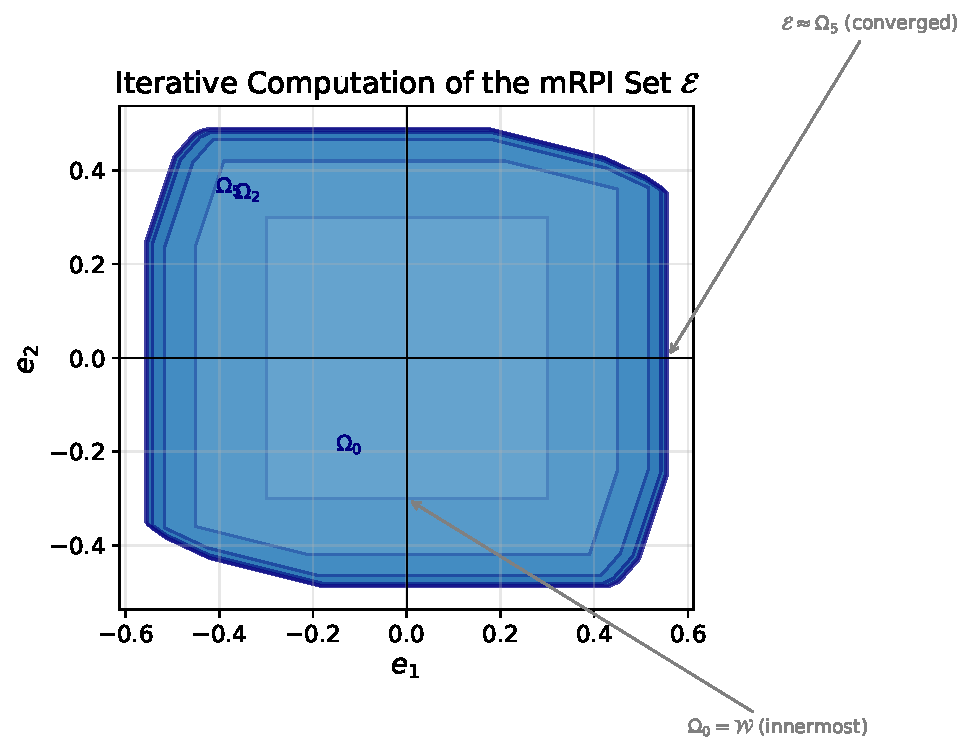
\includegraphics[width=0.6\linewidth]{Figures/mrpi_iteration.pdf}
	\caption{Iterative computation of the mRPI set. Starting from $\Omega_0 = \mathcal{W}$ (innermost set), each iteration adds a smaller and smaller set $A_{cl}^i\mathcal{W}$. The sets converge to the mRPI set $\mathcal{E}_\infty$.}
	\label{fig:mrpi_iteration}
\end{figure}

\textbf{The role of $K$.} A faster stabilising gain $K$ (one that places the eigenvalues of $A_{cl}$ closer to zero) produces a smaller mRPI set $\mathcal{E}_\infty$, because $A_{cl}^i\mathcal{W}$ shrinks faster. A smaller tube means less constraint tightening, which means a larger feasible region for the nominal MPC. However, aggressive gains require larger control inputs, which tightens the input constraints more. There is a trade-off in choosing $K$.

\begin{examplebox}{Computing the mRPI Set for a Scalar System}
	Consider the scalar system $x_{k+1} = 1.2\,x_k + u_k + w_k$ with $|w_k| \le 0.1$ and $|u_k| \le 1$. The stabilising gain is $K = 0.79$ (as returned by \texttt{dlqr}, so $u = -Kx$), giving $a_{cl} = 1.2 - 0.79 = 0.41$.

	\solution

	The mRPI set is the interval $\mathcal{E}_\infty = [-\bar{e}, \;\bar{e}]$, where:
	\[
	\bar{e} = \sum_{i=0}^{\infty} |a_{cl}|^i \cdot 0.1 = \frac{0.1}{1 - |a_{cl}|} = \frac{0.1}{1 - 0.41} = \frac{0.1}{0.59} \approx 0.169
	\]

	So the error $e_k = x_k - z_k$ is guaranteed to stay within $[-0.169, \; 0.169]$, no matter what disturbance sequence occurs (as long as $|w_k| \le 0.1$).

	\textbf{Constraint tightening.} If the original input constraint is $|u_k| \le 1$, the tightened input constraint for $v_k$ is:
	\[
	|v_k| \le 1 - |K| \cdot \bar{e} = 1 - 0.79 \times 0.169 \approx 0.867
	\]

	If the state constraint is $|x_k| \le 5$, the tightened state constraint for $z_k$ is:
	\[
	|z_k| \le 5 - 0.169 = 4.831
	\]

	The nominal MPC plans with these tighter bounds, and the feedback controller $u_k = v_k - K(x_k - z_k)$ takes care of the rest.
\end{examplebox}


\section{Step 4: Constraint Tightening}
\label{sec:constraint_tightening}

This is the central mechanism that makes Tube MPC robust. Since the real state $x_k = z_k + e_k$ can deviate from the nominal state $z_k$ by any amount in $\mathcal{E}$, we must ensure the constraints hold even in the worst case.

\textbf{State constraints.} We need $x_k = z_k + e_k \in \mathcal{X}$ for all $e_k \in \mathcal{E}$. This is equivalent to requiring:
\begin{equation}
	z_k \in \mathcal{X} \ominus \mathcal{E} \;=:\; \mathcal{X}_t
\end{equation}
The tightened state constraint set $\mathcal{X}_t$ is the original constraint set shrunk by the tube width.

\textbf{Input constraints.} The actual input is $u_k = v_k - Ke_k$. We need $u_k \in \mathcal{U}$ for all $e_k \in \mathcal{E}$. This gives:
\begin{equation}
	v_k \in \mathcal{U} \ominus K\mathcal{E} \;=:\; \mathcal{V}
\end{equation}
where $K\mathcal{E} = \{Ke \mid e \in \mathcal{E}\}$ is the set of all possible feedback corrections.

\textbf{Why does this work?} By construction:
\begin{itemize}[noitemsep]
	\item If $z_k \in \mathcal{X}_t$ and $e_k \in \mathcal{E}$, then $x_k = z_k + e_k \in \mathcal{X}$. \hfill (Definition of $\ominus$.)
	\item If $v_k \in \mathcal{V}$ and $e_k \in \mathcal{E}$, then $u_k = v_k - Ke_k \in \mathcal{U}$. \hfill (Definition of $\ominus$.)
\end{itemize}

The original hard constraints on $(x_k, u_k)$ are \emph{guaranteed} to be satisfied, regardless of which disturbance $w_k \in \mathcal{W}$ occurs. The price we pay is that the nominal trajectory has less room: the feasible region shrinks by the tube width on all sides.

\begin{notebox}{How much room do we lose?}
	The amount of constraint tightening depends directly on the size of $\mathcal{E}$, which in turn depends on:
	\begin{itemize}[noitemsep]
		\item \textbf{The disturbance bound $\mathcal{W}$}: Larger disturbances $\Rightarrow$ larger $\mathcal{E}$ $\Rightarrow$ more tightening.
		\item \textbf{The feedback gain $K$}: A faster gain shrinks $\mathcal{E}$ (less tightening of state constraints) but enlarges $K\mathcal{E}$ (more tightening of input constraints). A slower gain has the opposite effect.
	\end{itemize}

	In the extreme case where $\mathcal{W} = \{0\}$ (no disturbance), we get $\mathcal{E} = \{0\}$, and the tightened constraints equal the original constraints. Tube MPC reduces to standard MPC.
\end{notebox}


\section{Step 5: The Tube MPC Optimisation Problem}
\label{sec:tube_opt}

At each time step $k$, we measure the current state $x_k$ and solve the following optimisation over the nominal trajectory $(z, v)$:

\begin{equation} \label{eq:tube_mpc_opt}
	\begin{aligned}
		\min_{z_0, \ldots, z_N, \;\; v_0, \ldots, v_{N-1}} \quad & z_N^\top P\, z_N + \sum_{i=0}^{N-1} \bigl(z_i^\top Q\, z_i + v_i^\top R\, v_i\bigr) \\[6pt]
		\text{subject to:} \quad
		& z_{i+1} = Az_i + Bv_i, \qquad i = 0, \ldots, N-1 \\
		& z_i \in \mathcal{X}_t = \mathcal{X} \ominus \mathcal{E}, \qquad i = 0, \ldots, N-1 \\
		& v_i \in \mathcal{V} = \mathcal{U} \ominus K\mathcal{E}, \qquad i = 0, \ldots, N-1 \\
		& z_N \in \mathcal{X}_f \\
		& x_k \in z_0 \oplus \mathcal{E}
	\end{aligned}
\end{equation}

The key differences from standard MPC are:
\begin{enumerate}
	\item \textbf{The optimisation is over the nominal system} $(z, v)$, not the real system $(x, u)$. The nominal system has no disturbance, so this is a standard QP --- exactly the same type of problem we solved in Chapter~7.

	\item \textbf{The constraints are tightened.} The state and input constraints are shrunk inward by the tube width to account for the worst-case disturbance.

	\item \textbf{The initial condition links the nominal and real systems.} The constraint $x_k \in z_0 \oplus \mathcal{E}$ ensures the nominal starting point $z_0$ is close enough to the measured state $x_k$ that the error $e_0 = x_k - z_0$ lies within $\mathcal{E}$. In practice, this is often implemented by fixing $z_0 = x_k$ (which satisfies the constraint since $0 \in \mathcal{E}$), or by optimising over $z_0$ (which can improve performance by choosing a better tube centre).

	\item \textbf{The terminal set $\mathcal{X}_f$} is a positive invariant set for the nominal system under the tightened constraints, analogous to the terminal set in Chapter~7. It must satisfy $\mathcal{X}_f \subseteq \mathcal{X}_t$.
\end{enumerate}

After solving~\eqref{eq:tube_mpc_opt}, the control input applied to the real system is:
\begin{equation}
	u_k = v_0^\star - K(x_k - z_0^\star)
\end{equation}

At the next time step, we re-measure $x_{k+1}$ and solve again.


\section{Tube MPC Architecture}
\label{sec:tube_architecture}

The complete Tube MPC controller has the following structure:

\begin{center}
	\begin{tikzpicture}[
		block/.style={rectangle, rounded corners=4pt, draw=blue!60!black, fill=blue!8,
			text width=3.2cm, minimum height=1.2cm, align=center, font=\small\bfseries\sffamily},
		greenblock/.style={block, draw=green!50!black, fill=green!8},
		orangeblock/.style={block, draw=orange!60!black, fill=orange!8},
		arrow/.style={-Stealth, thick, draw=blue!60!black},
		]

		% Blocks
		\node[block] (mpc) {Nominal MPC\\(solves QP for $z$, $v$)};
		\node[orangeblock, right=2.5cm of mpc] (feedback) {Feedback\\$u = v_0^\star - K(x - z_0^\star)$};
		\node[greenblock, right=2.5cm of feedback] (plant) {Plant\\$x^+ = Ax + Bu + w$};

		% Offline block
		\node[block, below=1.5cm of mpc, text width=3.8cm] (offline) {Offline Computation\\$K$, $\mathcal{E}$, $\mathcal{X}_t$, $\mathcal{V}$, $\mathcal{X}_f$};

		% Arrows
		\draw[arrow] (mpc) -- node[above, font=\small\sffamily] {$v_0^\star, z_0^\star$} (feedback);
		\draw[arrow] (feedback) -- node[above, font=\small\sffamily] {$u_k$} (plant);
		\draw[arrow] (plant.south) -- ++(0,-0.8) -| node[below, near start, font=\small\sffamily] {$x_k$ (measured)} (mpc.south);
		\draw[arrow, dashed] (offline) -- (mpc);
	\end{tikzpicture}
\end{center}

The offline computation (feedback gain $K$, mRPI set $\mathcal{E}$, tightened constraints $\mathcal{X}_t$ and $\mathcal{V}$, and the terminal set $\mathcal{X}_f$) is performed once during the design phase. At run time, the controller only needs to solve the nominal QP (same size as standard MPC) and add the feedback correction.


\section{Worked Example: Tube MPC for a Scalar System}
\label{sec:tube_example_scalar}

\begin{examplebox}{Tube MPC: Scalar Integrator with Disturbance}
	Consider the system:
	\[
	x_{k+1} = 1.2\,x_k + u_k + w_k
	\]
	with $|u_k| \le 1$, $|x_k| \le 5$, $|w_k| \le 0.1$, and initial condition $x_0 = 2$.

	Design a Tube MPC controller with $Q = 1$, $R = 1$, $N = 5$.

	\solution

	\textbf{Step 1: Choose $K$ and compute the closed-loop eigenvalue.}

	Using the DARE with $Q = 1$, $R = 1$: $K = 0.79$ (positive, as returned by \texttt{dlqr}), so $u = -Kx \approx -0.79x$, giving $a_{cl} = a - bK = 1.2 - 0.79 = 0.41$.

	\textbf{Step 2: Compute the mRPI set.}
	\[
	\bar{e} = \frac{w_{\max}}{1 - |a_{cl}|} = \frac{0.1}{1 - 0.41} = \frac{0.1}{0.59} \approx 0.169
	\]
	So $\mathcal{E} = [-0.169, \; 0.169]$.

	\textbf{Step 3: Tighten constraints.}
	\begin{align*}
		\text{State:} \quad & |z_k| \le 5 - 0.169 = 4.831 \\
		\text{Input:} \quad & |v_k| \le 1 - |K| \cdot \bar{e} = 1 - 0.79 \times 0.169 \approx 0.867
	\end{align*}

	\textbf{Step 4: Solve the nominal MPC.}

	At each time step, solve the standard MPC problem~\eqref{eq:tube_mpc_opt} for the disturbance-free system $z_{k+1} = 1.2\,z_k + v_k$ with the tightened constraints $|z_k| \le 4.831$ and $|v_k| \le 0.867$.

	\textbf{Step 5: Apply the tube control law.}
	\[
	u_k = v_k^\star - K(x_k - z_k^\star) = v_k^\star - 0.79(x_k - z_k^\star)
	\]

	Figure~\ref{fig:tube_scalar} shows 50 different disturbance realisations. The blue traces are the actual state trajectories; the red dashed line is the nominal trajectory. All realisations remain within the constraint bounds, despite the disturbances.
\end{examplebox}

\begin{figure}[H]
	\centering
	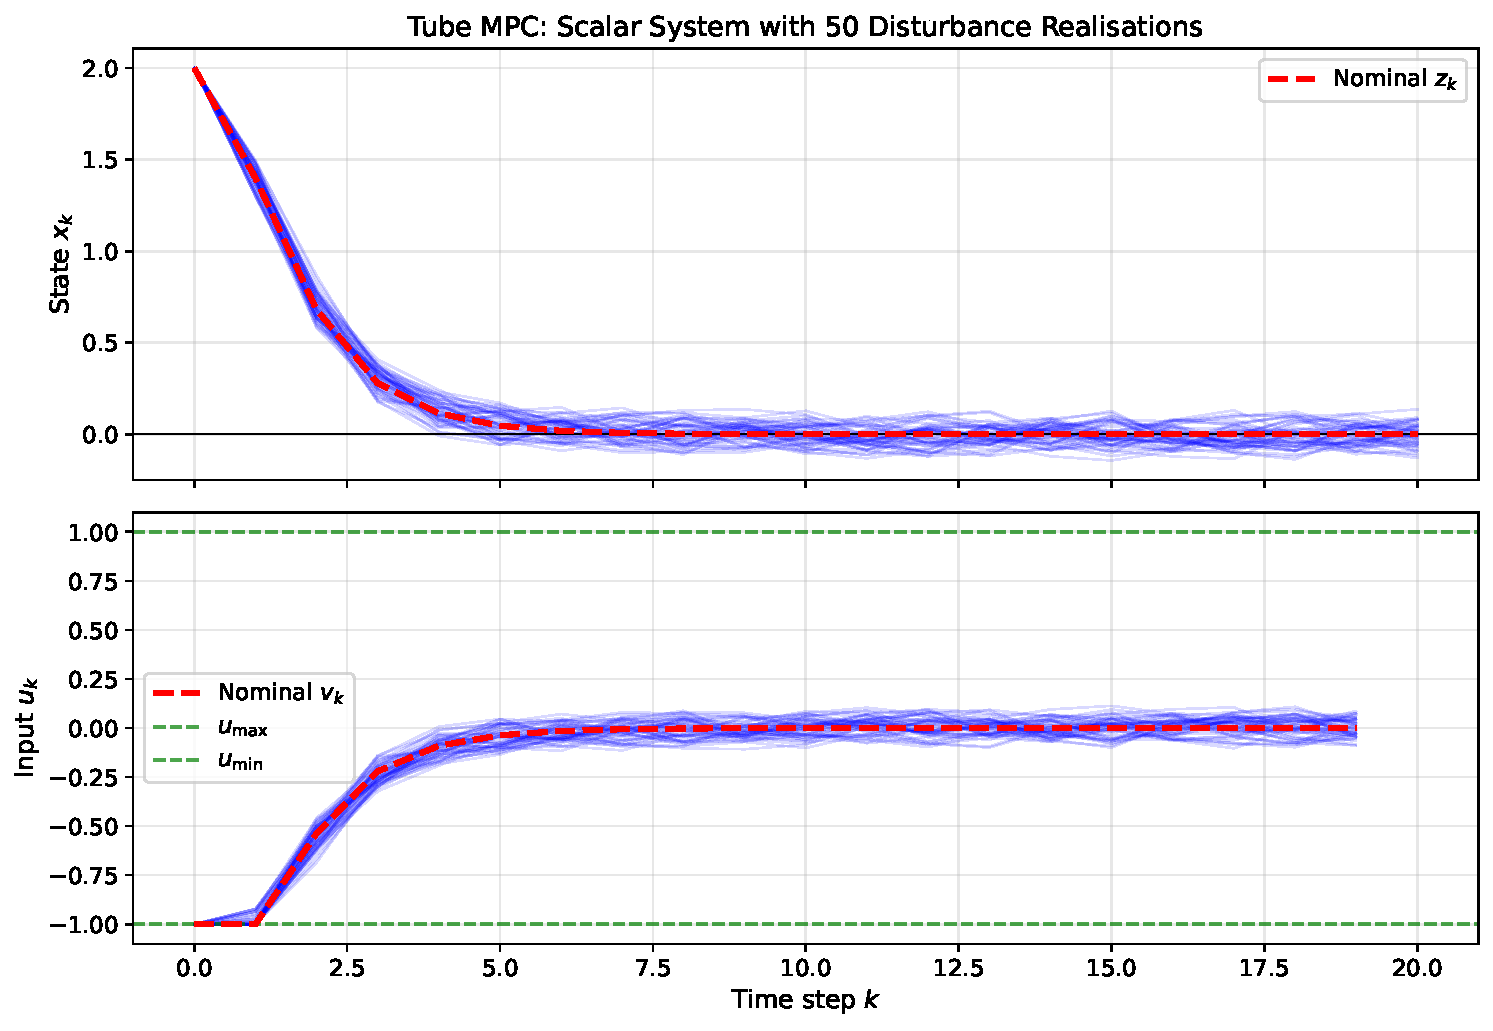
\includegraphics[width=0.85\linewidth]{Figures/tube_mpc_scalar.pdf}
	\caption{Tube MPC applied to the scalar system $x_{k+1} = 1.2\,x_k + u_k + w_k$ with $|w_k| \le 0.1$. Fifty disturbance realisations (blue) cluster around the nominal trajectory (red dashed). All trajectories satisfy the input constraints $|u_k| \le 1$.}
	\label{fig:tube_scalar}
\end{figure}


\section{Worked Example: Two-State System}
\label{sec:tube_example_2d}

\begin{examplebox}{Tube MPC: Double Integrator with Disturbance}
	Consider the double integrator:
	\[
	A = \begin{bmatrix} 1 & 1 \\ 0 & 1 \end{bmatrix}, \quad B = \begin{bmatrix} 0.5 \\ 1 \end{bmatrix}, \quad w_k \in \mathcal{W} = \{w \mid \|w\|_\infty \le 0.05\}
	\]
	with $|u_k| \le 1$, $|x_{1,k}| \le 5$, $|x_{2,k}| \le 3$, and $Q = I_2$, $R = 1$.

	\solution

	\textbf{Step 1: Compute LQR gain.}

	Solving the DARE gives $K = [0.4345 \;\; 1.0285]$ (positive, as returned by \texttt{dlqr}) and $P = \begin{bmatrix} 2.3671 & 1.1180 \\ 1.1180 & 2.5875 \end{bmatrix}$.

	The closed-loop matrix is:
	\[
	A_{cl} = A - BK = \begin{bmatrix} 1 - 0.2172 & 1 - 0.5142 \\ 0 - 0.4345 & 1 - 1.0285 \end{bmatrix} = \begin{bmatrix} 0.7828 & 0.4858 \\ -0.4345 & -0.0285 \end{bmatrix}
	\]
	The eigenvalues of $A_{cl}$ are approximately $0.377 \pm 0.216j$, with $|\lambda| \approx 0.434$, well inside the unit circle.

	\textbf{Step 2: Compute the mRPI set $\mathcal{E}$.}

	This requires the iterative Minkowski sum~\eqref{eq:mrpi}. For a two-state system, this is not practical by hand. Using MPT3 in MATLAB:

\begin{lstlisting}[language=Matlab]
A = [1 1; 0 1]; B = [0.5; 1];
Q = eye(2); R = 1;
[K_lqr, ~] = dlqr(A, B, Q, R);
Acl = A - B*K_lqr;

% Disturbance set
W = Polyhedron('lb', [-0.05; -0.05], 'ub', [0.05; 0.05]);

% Compute mRPI set (iterative Minkowski sum approximation)
% Note: invariantSet() computes the MAXIMAL positive invariant set,
% which is NOT the mRPI. The mRPI is computed via the iteration below.
Omega = W;
for i = 1:30
    Omega_new = Omega + (Acl^i) * W;  % Minkowski sum
    if Omega_new == Omega              % convergence check
        fprintf('mRPI converged at iteration %d\n', i);
        break;
    end
    Omega = Omega_new;
end
E = Omega;
\end{lstlisting}

	\textbf{Step 3: Tighten constraints.}
\begin{lstlisting}[language=Matlab]
X = Polyhedron('lb', [-5; -3], 'ub', [5; 3]);
U = Polyhedron('lb', -1, 'ub', 1);
KE = K_lqr * E;           % Image of E under K (set of |Ke| values)

Xt = X - E;               % Pontryagin difference
Vt = U - KE;              % Pontryagin difference
\end{lstlisting}

	\textbf{Step 4: Solve nominal MPC with tightened constraints.}

	The optimisation~\eqref{eq:tube_mpc_opt} is a standard QP with the same structure as Chapter~7. The only difference is that $\mathcal{X}$, $\mathcal{U}$ are replaced by $\mathcal{X}_t$, $\mathcal{V}$.

	\textbf{Step 5: Apply.} $u_k = v_0^\star - K(x_k - z_0^\star)$.
\end{examplebox}


\section{Guarantees of Tube MPC}
\label{sec:tube_guarantees}

Tube MPC provides three key guarantees, under the same type of assumptions as the nominal MPC stability theory (Chapter~7, Section~\ref{sec:mpc_stability_theory}).

\begin{summarybox}{Theorem: Properties of Tube MPC}
	Suppose $(A, B)$ is stabilisable, $K$ is chosen so that $A_{cl} = A - BK$ is Schur stable, and the MPC formulation~\eqref{eq:tube_mpc_opt} includes a terminal cost $P$ (DARE solution) and terminal set $\mathcal{X}_f$ for the nominal system. Then, for any disturbance sequence $\{w_k\} \subseteq \mathcal{W}$:
	\begin{enumerate}[noitemsep]
		\item \textbf{Robust constraint satisfaction:} The actual state and input satisfy $x_k \in \mathcal{X}$ and $u_k \in \mathcal{U}$ for all $k \ge 0$.
		\item \textbf{Recursive feasibility:} If the optimisation~\eqref{eq:tube_mpc_opt} is feasible at $k = 0$, it is feasible for all $k \ge 0$.
		\item \textbf{Robust stability:} The actual state converges to a neighbourhood of the origin. Specifically, $x_k$ converges to the mRPI set $\mathcal{E}$ (not to the origin itself, because the persistent disturbance prevents exact convergence).
	\end{enumerate}
\end{summarybox}

The first property follows directly from constraint tightening. The second uses the same shifted-sequence argument as in Chapter~7, applied to the nominal system. The third uses the nominal optimal cost $J^\star(z)$ as a Lyapunov function for the nominal system and then bounds the deviation of the real state.

Note a subtle difference from the nominal case: the state does not converge to zero. It converges to the mRPI set $\mathcal{E}$ around the origin. This is the best we can hope for with persistent disturbances --- we cannot drive the state to exactly zero when the disturbance keeps pushing it around.


\section{Tube MPC vs Standard MPC: A Comparison}
\label{sec:tube_comparison}

\begin{center}
	\begin{tabular}{L{4cm} C{4.5cm} C{4.5cm}}
		\toprule
		& \textbf{Standard MPC} & \textbf{Tube MPC} \\
		\midrule
		Model & $x_{k+1} = Ax_k + Bu_k$ & $x_{k+1} = Ax_k + Bu_k + w_k$ \\[3pt]
		Disturbance & Ignored & Bounded: $w_k \in \mathcal{W}$ \\[3pt]
		Constraint guarantee & Nominal only & Robust (for all $w \in \mathcal{W}$) \\[3pt]
		Online computation & Solve QP & Solve QP (same size) + feedback \\[3pt]
		Offline computation & $P$, $K$, $\mathcal{X}_f$ & $P$, $K$, $\mathcal{E}$, $\mathcal{X}_t$, $\mathcal{V}$, $\mathcal{X}_f$ \\[3pt]
		Convergence & $x_k \to 0$ & $x_k \to \mathcal{E}$ (neighbourhood of 0) \\[3pt]
		Feasible region & Larger & Smaller (due to tightening) \\
		\bottomrule
	\end{tabular}
\end{center}

The main takeaway: Tube MPC achieves robust guarantees at essentially no additional online cost. The extra work is in the offline design (computing $\mathcal{E}$ and tightening constraints), not in the real-time optimisation. The QP solved at each step has exactly the same size and structure as standard MPC.


\section{Implementation in MATLAB}
\label{sec:tube_matlab}

The following MATLAB code implements a complete Tube MPC simulation for the scalar system from Section~\ref{sec:tube_example_scalar}, using YALMIP.

\begin{lstlisting}[language=Matlab, caption={Tube MPC implementation for the scalar system}]
%% Tube MPC: Scalar System
% x_{k+1} = 1.2*x_k + u_k + w_k,  |w_k| <= 0.1
clear; clc;

%--- System parameters ---
a = 1.2;  b = 1;
Q = 1;    R = 1;    N = 5;

%--- Constraints ---
x_max = 5;   u_max = 1;   w_max = 0.1;

%--- Step 1: LQR gain ---
[K_lqr, P_dare] = dlqr(a, b, Q, R);
K = K_lqr;         % K > 0 (dlqr convention); control law: u = -K*x
a_cl = a - b*K;    % closed-loop eigenvalue: a_cl = a - b*K
fprintf('K = %.4f, a_cl = %.4f\n', K, a_cl);

%--- Step 2: mRPI set (scalar: geometric series) ---
e_bar = w_max / (1 - abs(a_cl));
fprintf('mRPI half-width: e_bar = %.4f\n', e_bar);

%--- Step 3: Tighten constraints ---
x_max_t = x_max - e_bar;              % tightened state
u_max_t = u_max - abs(K) * e_bar;     % tightened input
fprintf('Tightened: |z| <= %.3f, |v| <= %.3f\n', x_max_t, u_max_t);

%--- Step 4: Build nominal MPC with YALMIP ---
% z(1) is a decision variable (optimised), not fixed to x(k).
% Constraint: |x(k) - z(1)| <= e_bar (i.e., x(k) in {z(1)} + E).
z = sdpvar(1, N+1);   % nominal states (z(1) = z_0 is optimised)
v = sdpvar(1, N);      % nominal inputs
x_meas = sdpvar(1);   % parameter: measured state

constraints = [];
cost = 0;
for i = 1:N
    cost = cost + z(i)^2 * Q + v(i)^2 * R;
    constraints = [constraints, ...
        z(i+1) == a*z(i) + b*v(i), ...
        -x_max_t <= z(i) <= x_max_t, ...
        -u_max_t <= v(i) <= u_max_t];
end
cost = cost + z(N+1)^2 * P_dare;  % terminal cost
constraints = [constraints, -x_max_t <= z(N+1) <= x_max_t];

% Tube constraint: x(k) must lie in {z_0} + E
constraints = [constraints, -e_bar <= x_meas - z(1) <= e_bar];

params_in = x_meas;          % parameter: measured state
sols_out = [v(1), z(1)];     % solutions: first nominal input AND z_0

ops = sdpsettings('verbose', 0, 'solver', 'quadprog');
controller = optimizer(constraints, cost, ops, params_in, sols_out);

%--- Step 5: Simulate ---
T_sim = 30;
x = zeros(1, T_sim+1);
z_traj = zeros(1, T_sim+1);
u_applied = zeros(1, T_sim);

x(1) = 2.0;      % initial condition

rng(42);
for k = 1:T_sim
    % Solve nominal MPC (z_0 is optimised, not fixed to x(k))
    sol = controller(x(k));
    v0 = sol(1);
    z0 = sol(2);

    % Apply tube control law: u = v - K*(x - z)
    % Note: z0 ~= x(k) in general, so the feedback term is nonzero
    u_applied(k) = v0 - K * (x(k) - z0);
    u_applied(k) = max(-u_max, min(u_max, u_applied(k)));

    % Simulate real system with disturbance
    w = w_max * (2*rand - 1);   % uniform in [-w_max, w_max]
    x(k+1) = a * x(k) + b * u_applied(k) + w;

    % Store nominal trajectory for plotting
    z_traj(k) = z0;
    z_traj(k+1) = a * z0 + b * v0;
end

%--- Plot ---
figure;
subplot(2,1,1);
plot(0:T_sim, x, 'b-', 'LineWidth', 1.5); hold on;
plot(0:T_sim, z_traj, 'r--', 'LineWidth', 1.5);
yline(x_max, 'g--'); yline(-x_max, 'g--');
ylabel('State'); legend('Actual x_k', 'Nominal z_k', 'Constraint');
title('Tube MPC: Scalar System'); grid on;

subplot(2,1,2);
stairs(0:T_sim-1, u_applied, 'b-', 'LineWidth', 1.5);
yline(u_max, 'g--'); yline(-u_max, 'g--');
xlabel('Time step k'); ylabel('Input u_k');
legend('Applied input', 'Constraint'); grid on;
\end{lstlisting}


\section{Computing the mRPI Set with MPT3}
\label{sec:tube_mpt3}

For multi-state systems, computing the mRPI set by hand is impractical. The MPT3 toolbox~\cite{Herceg2013} provides automated tools for this. The key steps are:

\begin{lstlisting}[language=Matlab, caption={Computing the mRPI set and tightened constraints using MPT3}]
%% Tube MPC Offline Design using MPT3
% System: x+ = Ax + Bu + w,  w in W

A = [1 1; 0 1];   B = [0.5; 1];
Q = eye(2);        R = 1;

% LQR gain
[K_lqr, P_dare] = dlqr(A, B, Q, R);
Acl = A - B*K_lqr;

% Define constraint sets as Polyhedra
X = Polyhedron('lb', [-5; -3], 'ub', [5; 3]);     % state
U = Polyhedron('lb', -1, 'ub', 1);                 % input
W = Polyhedron('lb', [-0.05; -0.05], ...
               'ub', [0.05; 0.05]);                 % disturbance

% --- Compute the mRPI set ---
% Iterative Minkowski sum: E = W + Acl*W + Acl^2*W + ...
E = W;
for i = 1:30
    E_new = E + Acl^i * W;   % Minkowski sum
    if E_new == E             % convergence check
        fprintf('mRPI converged at iteration %d\n', i);
        break;
    end
    E = E_new;
end
\end{lstlisting}

\begin{notebox}{Convergence check}
The equality test \texttt{E\_new == E} uses MPT3's polytope comparison, which involves solving linear programmes.  For production code, a tolerance-based criterion (e.g.\ comparing support functions or Hausdorff distances) is more numerically robust.  The outer-approximation algorithm of \citet{Rakovic2005} provides explicit error bounds.
\end{notebox}

\begin{lstlisting}[language=Matlab]

% --- Tighten constraints ---
KE  = K_lqr * E;        % image of E under gain K (set of |Ke| values)
Xt  = X - E;             % Pontryagin difference: X ominus E
Vt  = U - KE;            % Pontryagin difference: U ominus KE

% --- Compute terminal set for nominal system ---
sys_nom = LTISystem('A', A - B*K_lqr);
% NOTE: Xt.Internal.lb/ub exist because X and E are both boxes (hyperrectangles).
% For general polytopic constraints, use Xt.A and Xt.b with LTISystem's setConstraint method.
sys_nom.x.min = Xt.Internal.lb;
sys_nom.x.max = Xt.Internal.ub;
Xf = sys_nom.invariantSet();

% --- Extract half-space representation for QP ---
% Tightened state: Xt.A * z <= Xt.b
% Tightened input: Vt.A * v <= Vt.b
% Terminal:        Xf.A * z_N <= Xf.b

fprintf('Tightened state constraints: %d inequalities\n', size(Xt.A, 1));
fprintf('Tightened input constraints: %d inequalities\n', size(Vt.A, 1));
fprintf('Terminal set: %d inequalities\n', size(Xf.A, 1));
\end{lstlisting}

\begin{notebox}{Approximate mRPI for large systems}
	For systems with more than 3--4 states, the exact mRPI computation can produce polytopes with a very large number of faces, making the resulting QP expensive. In practice, an outer approximation $\hat{\mathcal{E}} \supseteq \mathcal{E}_\infty$ is often used instead~\cite{Rakovic2005}. A common approach is to stop the iteration after a fixed number of steps $s$ and scale the result slightly outward: $\hat{\mathcal{E}} = (1-\epsilon)^{-1}\,\Omega_s$ for a small $\epsilon > 0$ chosen so that $A_{cl}^{s+1}\mathcal{W} \subseteq \epsilon\,\Omega_s$. This guarantees that $\hat{\mathcal{E}}$ is a true RPI set while keeping the number of polytope faces manageable.
\end{notebox}


\section{Visualising the Tube}
\label{sec:tube_visualisation}

Figure~\ref{fig:tube_concept} illustrates the key concept. The nominal trajectory $z_k$ (red dashed) is planned by the MPC optimiser. The actual trajectory $x_k$ (blue solid) deviates due to disturbances but stays within the grey ``tube'' --- the Minkowski sum $\{z_k\} \oplus \mathcal{E}$ at each step. The nominal trajectory respects the tightened constraints (orange lines), which guarantees the actual trajectory respects the original constraints (green dashed lines).

\begin{figure}[H]
	\centering
	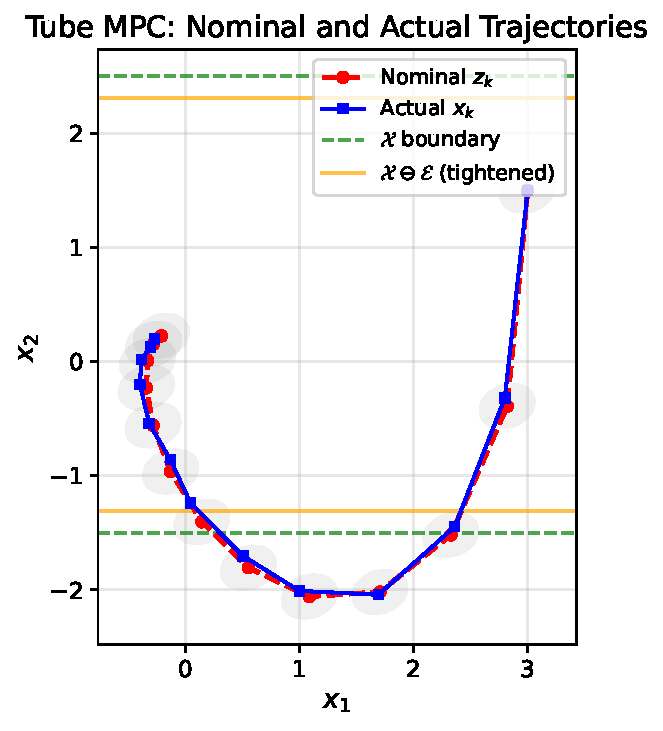
\includegraphics[width=0.85\linewidth]{Figures/tube_mpc_concept.pdf}
	\caption{The tube concept in state space. Grey ellipses represent the cross-section $\mathcal{E}$ of the tube at each time step. The nominal trajectory (red) stays within the tightened constraints (orange), ensuring the actual trajectory (blue) stays within the original constraints (green dashed).}
	\label{fig:tube_concept}
\end{figure}


\section{Summary and Practical Guidelines}

\begin{summarybox}{Tube MPC Design Recipe}
	\begin{enumerate}
		\item \textbf{Model the disturbance.} Identify the disturbance set $\mathcal{W}$ from physical knowledge or data. Larger $\mathcal{W}$ gives more robustness but tighter constraints.

		\item \textbf{Choose the feedback gain $K$.} Use LQR or pole placement. Faster gains give a smaller tube (less constraint tightening) but require more control effort (more input constraint tightening). There is a design trade-off.

		\item \textbf{Compute the mRPI set $\mathcal{E}$.} Use the iterative Minkowski sum~\eqref{eq:mrpi} or MPT3. For scalar systems, use the geometric series formula.

		\item \textbf{Tighten constraints.} State: $\mathcal{X}_t = \mathcal{X} \ominus \mathcal{E}$. Input: $\mathcal{V} = \mathcal{U} \ominus K\mathcal{E}$. Check that the tightened sets are non-empty; if they are empty, the disturbance is too large relative to the constraints, and robust constraint satisfaction is impossible.

		\item \textbf{Design the nominal MPC.} Solve a standard MPC problem with the tightened constraints. All the techniques from Chapter~7 apply (terminal cost $P$, terminal set $\mathcal{X}_f$, YALMIP implementation).

		\item \textbf{Apply the tube law.} At each step: $u_k = v_0^\star - K(x_k - z_0^\star)$.
	\end{enumerate}
\end{summarybox}

\begin{alertbox}{When Tube MPC cannot help}
	If the disturbance bound $\mathcal{W}$ is so large that the tightened constraint sets $\mathcal{X}_t$ or $\mathcal{V}$ become empty, then no controller can guarantee robust constraint satisfaction. In this case, the system physically cannot respect the constraints under all possible disturbances. Options include: relaxing the constraints (soft constraints), reducing the disturbance (better actuators or shielding), or accepting occasional constraint violations and using a stochastic MPC approach instead.
\end{alertbox}


\section*{Further Reading}

The Tube MPC framework was introduced by Langson et al.~\cite{Langson2004} and further
developed by Mayne et al.~\cite{Mayne2005}. The efficient outer approximation of the
mRPI set used in practice is due to Rakovi{\'c} et al.~\cite{Rakovic2005}. For a
comprehensive treatment of robust MPC including stochastic formulations, see
Kouvaritakis and Cannon~\cite{Kouvaritakis2016}. The broader MPC stability theory
underpinning the guarantees discussed in this chapter is surveyed in
Mayne et al.~\cite{Mayne2000}. The textbooks by Rawlings et al.~\cite{Rawlings2017}
and Borrelli et al.~\cite{Borrelli2017} provide detailed treatments of both nominal
and robust MPC.

\section*{Exercises}
\begin{enumerate}

	\item Consider the scalar system $x_{k+1} = 1.5\,x_k + u_k + w_k$ with $|u_k| \le 2$, $|w_k| \le 0.2$, and $Q = R = 1$.
	\begin{enumerate}
		\item Compute the LQR gain $K$ and the closed-loop eigenvalue $a_{cl}$.
		\item Using the geometric series formula, compute the mRPI half-width $\bar{e}$.
		\item What are the tightened input constraints for the nominal MPC?
		\item If $|x_k| \le 10$, what are the tightened state constraints?
	\end{enumerate}

	\item Compute the Minkowski sum $P \oplus Q$ and the Pontryagin difference $P \ominus Q$ for:
	\begin{enumerate}
		\item $P = [-3, 3]$, $Q = [-1, 1]$ (intervals in $\mathbb{R}$).
		\item $P = \{(x_1, x_2) \mid |x_1| \le 2, |x_2| \le 2\}$ (a square) and $Q = \{(x_1, x_2) \mid |x_1| + |x_2| \le 0.5\}$ (a diamond). Sketch the results.
	\end{enumerate}

	\item A control engineer designs Tube MPC for a chemical process with $|w_k| \le 0.5$ and input constraint $|u_k| \le 3$. The LQR gain is $K = 1.8$ (positive, with $u = -Kx$) and the closed-loop eigenvalue is $a_{cl} = 0.3$.
	\begin{enumerate}
		\item Compute the tube width $\bar{e}$.
		\item What is the tightened input constraint for $v_k$?
		\item The engineer's colleague suggests using a more aggressive gain with $a_{cl} = 0.1$, which gives $K = 2.5$. Recompute the tube width and tightened input constraint. Is this gain better or worse? Discuss the trade-off.
	\end{enumerate}

	\item Consider the double integrator from Section~\ref{sec:tube_example_2d}. Using MATLAB and MPT3:
	\begin{enumerate}
		\item Compute the mRPI set $\mathcal{E}$ for $\mathcal{W} = \{w \mid \|w\|_\infty \le 0.05\}$.
		\item Plot the original constraint set $\mathcal{X}$, the mRPI set $\mathcal{E}$, and the tightened constraint set $\mathcal{X}_t = \mathcal{X} \ominus \mathcal{E}$.
		\item Repeat with $\mathcal{W} = \{w \mid \|w\|_\infty \le 0.2\}$. How does the larger disturbance affect the feasible region?
		\item Find the largest disturbance bound $\delta$ such that $\mathcal{X}_t$ is still non-empty (i.e., the tightened constraint set has positive volume).
	\end{enumerate}

	\item Explain in your own words:
	\begin{enumerate}
		\item Why does Tube MPC guarantee convergence to a neighbourhood of the origin rather than to the origin itself?
		\item What happens to the tube width $\mathcal{E}$ as the feedback gain $K$ becomes more aggressive (eigenvalues of $A_{cl}$ closer to zero)?
		\item Under what conditions does Tube MPC reduce to standard MPC?
	\end{enumerate}

\end{enumerate}
